\documentclass[12pt]{article}
\usepackage{graphicx}
\usepackage[margin=1in]{geometry}
\usepackage{caption}
\usepackage{float}
\usepackage{amsmath}
\usepackage{array}
\usepackage{multicol}
\usepackage{hyperref}
\usepackage{url}

\setlength{\columnsep}{1cm}

\begin{document}

% Title Block
\begin{center}
    \textbf{\Large IMPLEMENTATION OF UGV THROUGH BLUETOOTH VOICE COMMAND AND WIFI BASED WEB CONTROL} \\[10pt]
    \textbf{Ch.Pranai} \\
   % \texttt{pranaichatakondu@gmail.com} \\
   % \textbf{COMET.FWC022} \\
    \textbf{Future Wireless Communication (FWC)} \\
    \textbf{ASSIGNMENT} \\[5pt]
    July 18, 2025
\end{center}
\vspace{1em}

\begin{multicols}{2}

% Abstract
\noindent\textbf{Abstract} \\[0.5em]
\noindent This project implements a voice-controlled Unmanned Ground Vehicle (UGV) using an ESP32 microcontroller.Voice commands are captured via a mobile app and sent to the ESP32 over Bluetooth.The ESP32 interprets these commands to control motor movements like forward, backward, left, and right.A secondary control option is provided via a Wi-Fi-based web interface.The system enables hands-free, wireless control suitable for smart robotics and automation tasks.\\

\vspace{1em}
\noindent\textbf{1. Components}
\begin{table}[H]
\small
\centering
\begin{tabular}{|p{4.2cm}|c|}
\hline
\textbf{Component} & \textbf{Qty} \\
\hline
ESP32  Board & 1 \\
L298N Motor control & 1\\
UGV Car Kit & 1 \\
USB Cable (Type C) & 1 \\
Jumper Wires (F-F) & 8 \\
Android Mobile with RoboBoy App & 1 \\
Batteries(1.5v) & 4\\
\hline
\end{tabular}
\caption*{Table 1: List of components used}
\end{table}

\vspace{1em}
\noindent\textbf{2. Setup and Connections}
\begin{enumerate}
    \item Assemble the toy car according to the instructions in  manual.
    \item Make the connections according to the Schematic diagram.
    \item Make sure connect the Vin pin of ESP32 board to Vms terminal of L298N.
    \item If we want to control via Bluetooth through RoboBoy App, we need to create a project inside the app to meet our requirements like giving audio for commands like  "forward", "backward","left","right","stop".
\end{enumerate}

\vspace{1em}
\noindent\textbf{3. Steps for Implementation}
\begin{enumerate}
    \item Open tools in arduino ide select ESP32Devmodule in "Boards", select port "devttyUSB0".
    \item Also in tools select Partition Scheme: "Minimal SPIFFS (1.9MB APP with OTA/190KB SPIFFS)" otherwise we may face problem while uploading.
    \item Compile and upload the code into ESP32 board via USB cable .
    \item After uploading remove the cable and connect the vehicle either with bluetooth using RoboBoy app or with wifi.
\end{enumerate}

\vspace{1em}

\end{multicols}
\vspace{4em}
\vspace{1em}
\begin{multicols}{2}
\begin{figure}[H]
    \centering
    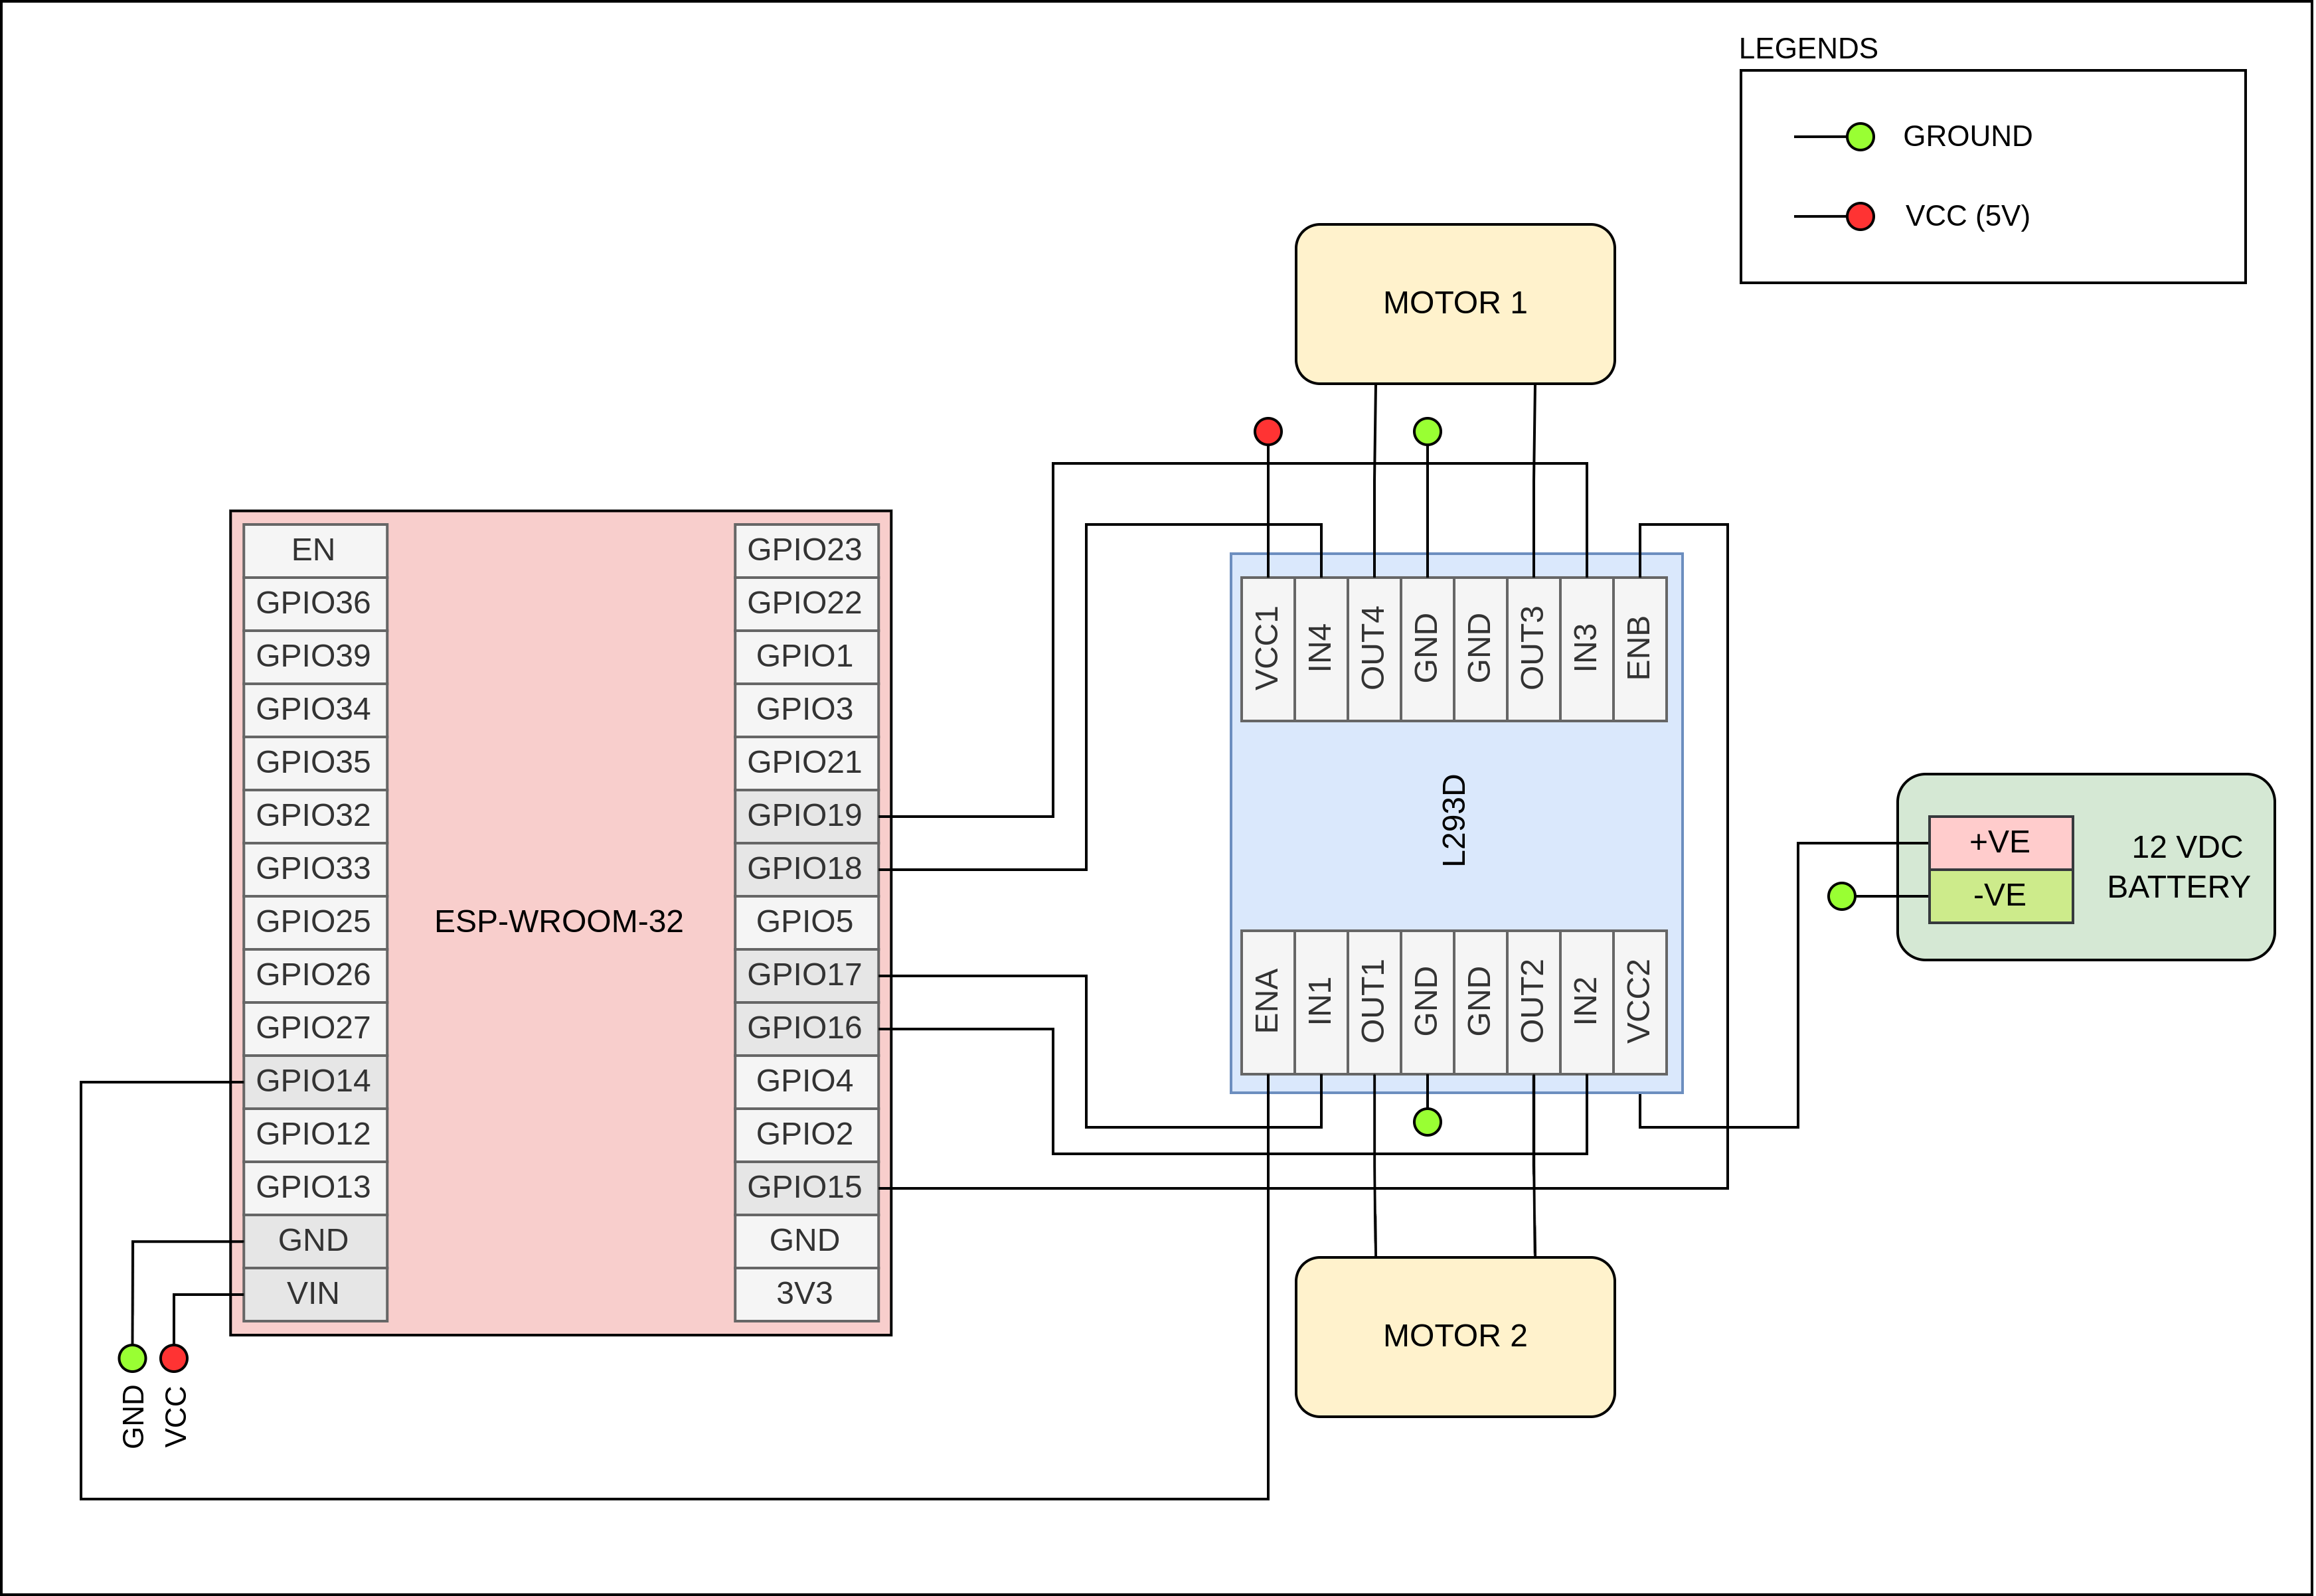
\includegraphics[width=0.9\linewidth]{BWUGV.png}
    \caption{Schematic Diagram.}
    \label{fig:image1}
\end{figure}

\end{multicols}
\end{document}
